Ce chapitre décrit les technologies ainsi que les méthodes d'analyses qui seront utilisées dans le cadre de ce projet.

\section{Technologies}

Afin de mettre en place ce projet, différentes technologies vont être utilisées.

Pour la récupération des données, nous allons utiliser le langage de programmation \textbf{Python} avec les librairies
\textbf{Scrapy}, \textbf{BeautifulSoup} et \textbf{Selenium}. Ces différentes données seront stockées dans une base de données \textbf{MongoDB}. 
Cela facilitera la gestion car elles seront stockées sous forme de documents JSON.
Afin d'être utilisables ces données seront servies par une API REST en utilisant \textbf{FastAPI}.
Pour finir une application web sera développée en le framework \textbf{ReactJS}.

En résumé, la stack technologique utilisée est la suivante: 
\begin{itemize}
    \item \textbf{Python} pour la récupération des données.
    \item \textbf{Scrapy}, \textbf{BeautifulSoup} et \textbf{Selenium} pour la récupération des données.
    \item \textbf{MongoDB} pour le stockage des données.
    \item \textbf{ExpressJS} pour la création de l'API REST.
    \item \textbf{ReactJS} pour la création de l'application web.
\end{itemize}   

Le diagramme de la figure \ref{fig:architecture} illustre l'architecture globale du projet.

\begin{figure}[H]
    \centering
    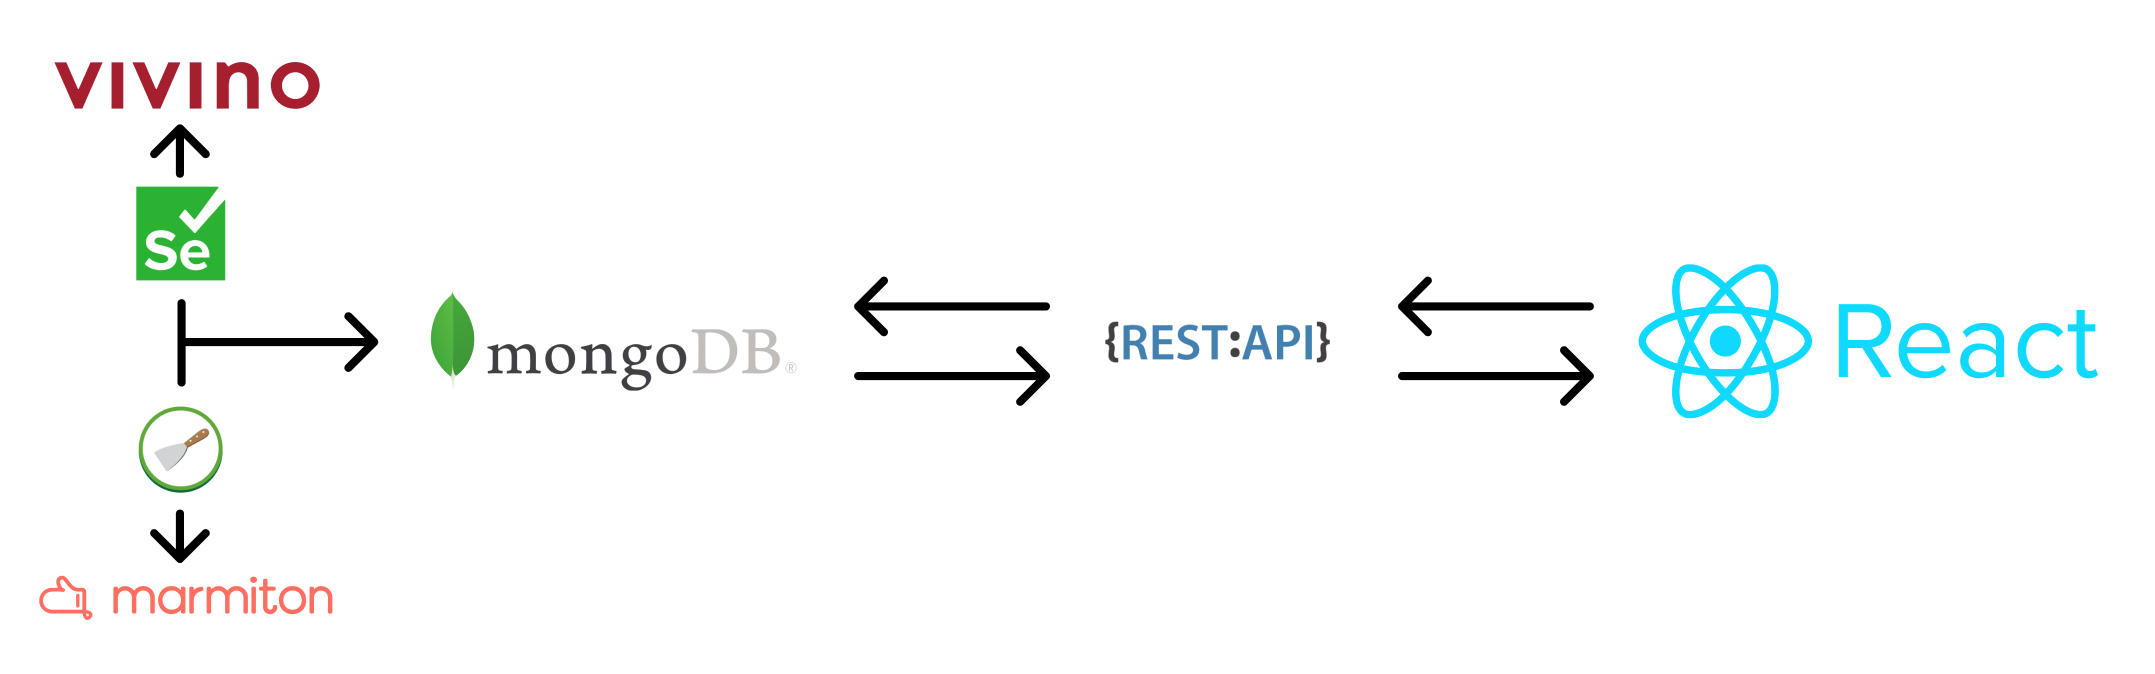
\includegraphics[width=0.8\textwidth]{rsc/architecture.png}
    \caption{Architecture globale du projet.}
    \label{fig:architecture}
\end{figure}


\section{Méthodes d'analyse}

Deux méthodes d'analyse sont envisagés dans ce projet. La première doit permettre recommander un vin pour une recette en comparant les listes d'accords des vins avec le nom et les ingrédients de la recette. La seconde doit permettre de déterminer si le vin est apprécié et les points qui le caractérisent en analysant les commentaires des utilisateurs sur les vins.

\subsection{Recommandation de vin}

Afin de recommander un vin suivant une recette, nous allons générer pour chaque recette une liste de vecteurs représentant son nom et ses ingrédients à l'aide d'un générateur d'embedding de mots comme Word2Vec ou GloVe. Pour chaque vin, nous procéderons de la même manière en générant une liste de vecteurs représentant les plats avec lesquels il s'accorde. La figure \ref{fig:word2vec} illustre la génération de ces vecteurs et leur stockage dans la base de données. Cette génération sera donc effectuée qu'une seule fois, sur toutes les données récupérées.

Ces vecteurs étant persistés dans la base, il sera possible de les récupérer une fois que l'utilisateur aura sélectionné une recette. Les similarités (par exemple la similarité cosinus) entre les vecteurs de la recette et ceux des vins seront ensuite calculées puis moyennées pour obtenir une note de recommandation. Une liste contenant les meilleurs vins s'accordant avec la recette sera alors retournée à l'utilisateur. La figure \ref{fig:recommandation} illustre ce processus.

% \begin{figure}[H]
%     \centering
%     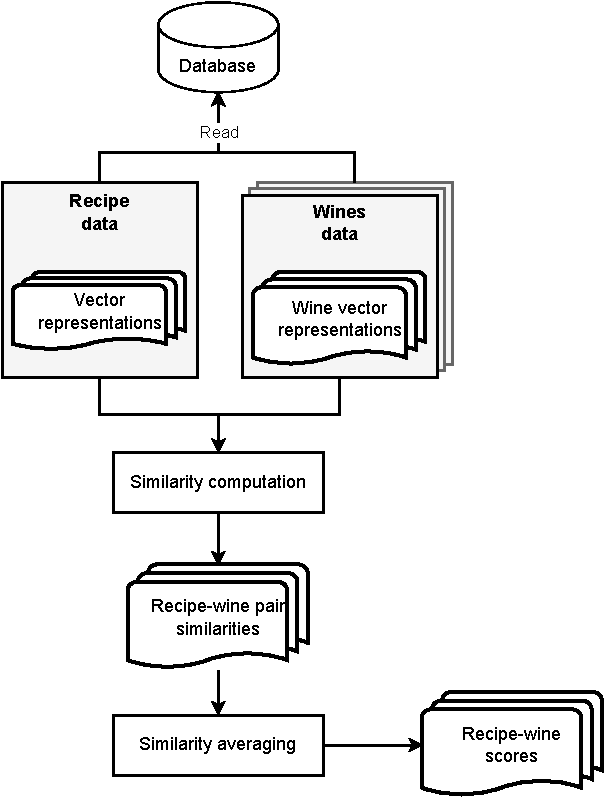
\includegraphics[width=0.4\textwidth]{rsc/similarities.pdf}
%     \caption{Processus de recommandation d'un vin pour une recette.}
%     \label{fig:recommandation}
% \end{figure}

\begin{figure}[H]
    \centering
    \begin{minipage}[b]{.5\textwidth}
      \centering
      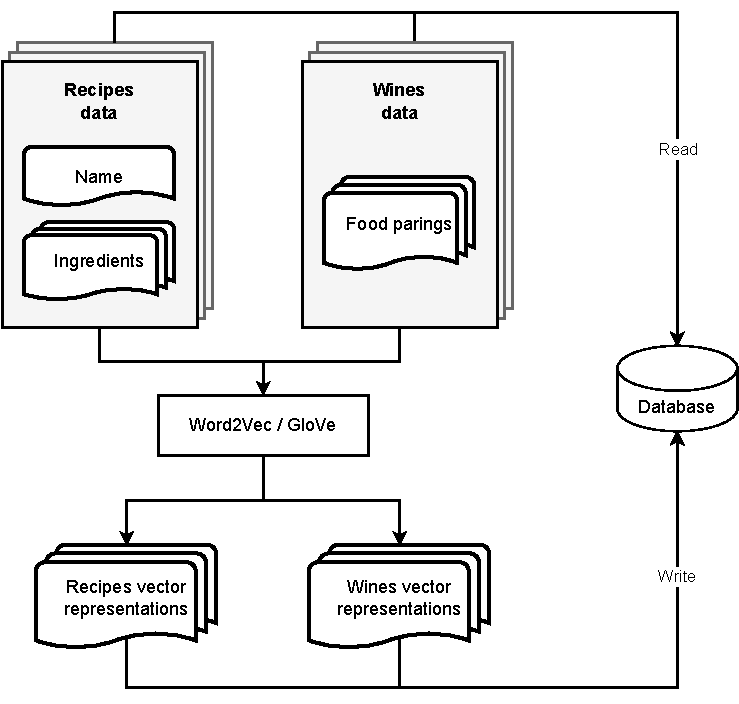
\includegraphics[width=.8\linewidth]{rsc/embedding_generation.pdf}
      \caption{\centering Processus de génération et de stockage des vecteurs représentatifs.}
      \label{fig:word2vec}
    \end{minipage}%
    \begin{minipage}[b]{.5\textwidth}
      \centering
      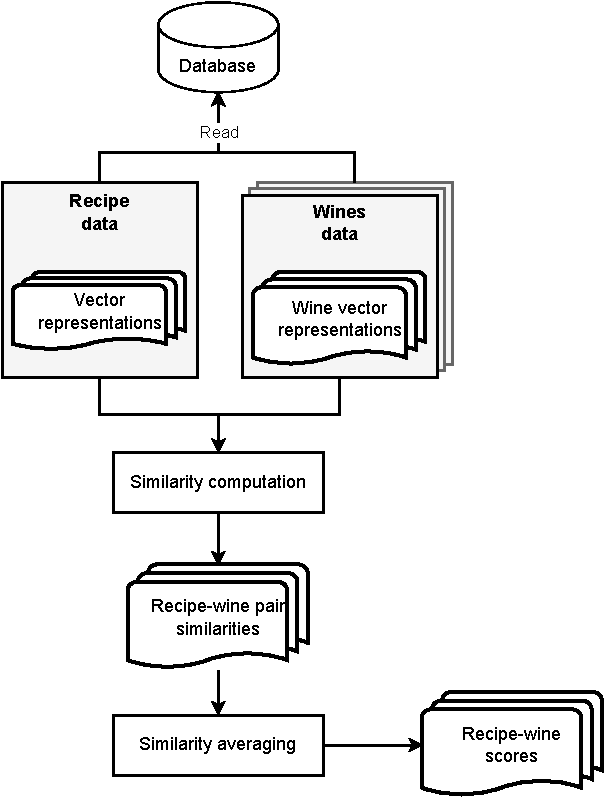
\includegraphics[width=.8\linewidth]{rsc/similarities.pdf}
      \caption{\centering Processus de recommandation d'un vin pour une recette.}
      \label{fig:recommandation}
    \end{minipage}
    \end{figure}

\subsection{Analyse des commentaires}
Afin d'analyser les commentaires, nous allons utiliser la librairie Python "pysentimiento". Cette librairie se base sur des modèles d'apprentissage profond Transformeur pour réaliser des tâches de traitement du langage naturel. Elle permet notamment de classifier un texte (dans notre cas le cas un commentaire) selon s'il est de nature positive, neutre ou négative, et également de générer le sentiment principal qui en ressort comme la joie, la tristesse ou encore la colère.
